\documentclass[aspectratio=169,11pt]{beamer}
\usetheme{default}
\usefonttheme{professionalfonts}

\usepackage[utf8]{inputenc}
\usepackage{amsmath,amssymb}
\usepackage{booktabs}
\usepackage{graphicx}
\graphicspath{{figures/}}
\usepackage{tikz}
\usetikzlibrary{arrows.meta, positioning, shapes.geometric, backgrounds, fit, calc}

% ==============================================================================
% COLOR PALETTE & DESIGN SYSTEM
% Clean, modern academic theme: Deep navy primary, clean white canvas,
% muted red for explosions, muted blue for earthquakes, teal accent.
% ==============================================================================
\definecolor{navy}{RGB}{11, 27, 61}          % #0B1B3D - Deep primary navy
\definecolor{blastred}{RGB}{197, 48, 48}     % #C53030 - Muted explosion red
\definecolor{quakeblue}{RGB}{43, 108, 176}   % #2B6CB0 - Muted earthquake blue
\definecolor{tealaccent}{RGB}{13, 148, 136}  % #0D9488 - Modern teal accent
\definecolor{slate}{RGB}{100, 116, 139}      % #64748B - Muted slate text
\definecolor{lightbg}{RGB}{248, 250, 252}    % #F8FAFC - Soft panel background
\definecolor{bordergray}{RGB}{226, 232, 240} % #E2E8F0 - Divider line
\definecolor{lightgreen}{RGB}{220, 252, 231} % Soft highlight green

% Remove navigation symbols
\setbeamertemplate{navigation symbols}{}

% Even margins around each slide (0.8cm left and right)
\setbeamersize{text margin left=0.8cm, text margin right=0.8cm}

% Clean frame titles
\setbeamercolor{frametitle}{fg=navy,bg=white}
\setbeamerfont{frametitle}{series=\bfseries,size=\large}
\setbeamertemplate{frametitle}{
  \vspace*{0.6cm}
  \centering\insertframetitle\par
  \vspace*{0.2cm}
}

% Clean minimal footer: slide number only
\setbeamertemplate{footline}{
  \ifnum\thepage>1
    \hfill \footnotesize\color{slate}\insertframenumber{} / \inserttotalframenumber \hspace*{0.8cm}\vspace*{0.35cm}
  \fi
}

% Clean list styling
\setbeamertemplate{itemize item}{\color{tealaccent}\textbf{\rule[0.5ex]{0.7ex}{0.7ex}}}
\setbeamertemplate{itemize subitem}{\color{slate}\textbf{--}}
\setlength{\leftmargini}{1.1em}

% Metadata
\title{Discriminating Underground Nuclear Explosions from Natural Earthquakes}
\subtitle{Using Signal Processing and Machine Learning Methods}
\author{Rajveer Vora \and Smarak Patel \and Tanish Ghosh}
\institute{ASM-II Course Project $\cdot$ Indian Statistical Institute}
\date{November 2026}

\begin{document}

% ==============================================================================
% SLIDE 1: TITLE SLIDE (Dark Navy Impact Style)
% ==============================================================================
{
\setbeamercolor{background canvas}{bg=navy}
\begin{frame}[plain]
  \vspace*{0.75cm}
  \centering
  {\fontsize{22}{26}\selectfont \textbf{\color{white} Discriminating Underground Nuclear Explosions\\[0.25em] from Natural Earthquakes}}\\[0.8em]
  {\fontsize{12}{15}\selectfont \color{tealaccent} Using Signal Processing and Machine Learning Methods}\\[1.8em]

  {\fontsize{11}{14}\selectfont \color{white}
    \textbf{Rajveer Vora} (ISIK) \qquad
    \textbf{Smarak Patel} (ISID) \qquad
    \textbf{Tanish Ghosh} (ISIB)
  }\\[0.9em]

  {\fontsize{10}{12}\selectfont \color{slate}
    ASM-II Course Project $\cdot$ Indian Statistical Institute\\[0.3em]
    November 2026
  }
\end{frame}
}

% ==============================================================================
% SLIDE 2: MOTIVATING TIME-FREQUENCY REPRESENTATIONS
% ==============================================================================
\begin{frame}{Motivating Time-Frequency Representations}
  \centering{\small \color{slate} Raw amplitudes overlap; time-varying frequency content provides the primary statistical discriminant.}\par
  \vspace*{0.05cm}

  \begin{columns}[T,onlytextwidth]
    \begin{column}{0.315\textwidth}
      \textbf{\color{navy} 1. Amplitude Ambiguity}\\[0.1em]
      \footnotesize 1D waveforms overlap in amplitude and envelope; magnitude alone cannot classify the source.
    \end{column}
    \hfill
    \begin{column}{0.325\textwidth}
      \textbf{\color{navy} 2. Spectral Evolution}\\[0.1em]
      \footnotesize Blasts concentrate high frequencies early; earthquakes sustain lower frequencies in late coda.
    \end{column}
    \hfill
    \begin{column}{0.315\textwidth}
      \textbf{\color{navy} 3. 2D Tensor Mapping}\\[0.1em]
      \footnotesize \textbf{STFT} maps 1D temporal series into 2D time-frequency grids for feature extraction and CNNs.
    \end{column}
  \end{columns}

  \vspace*{0.05cm}
  \centering
  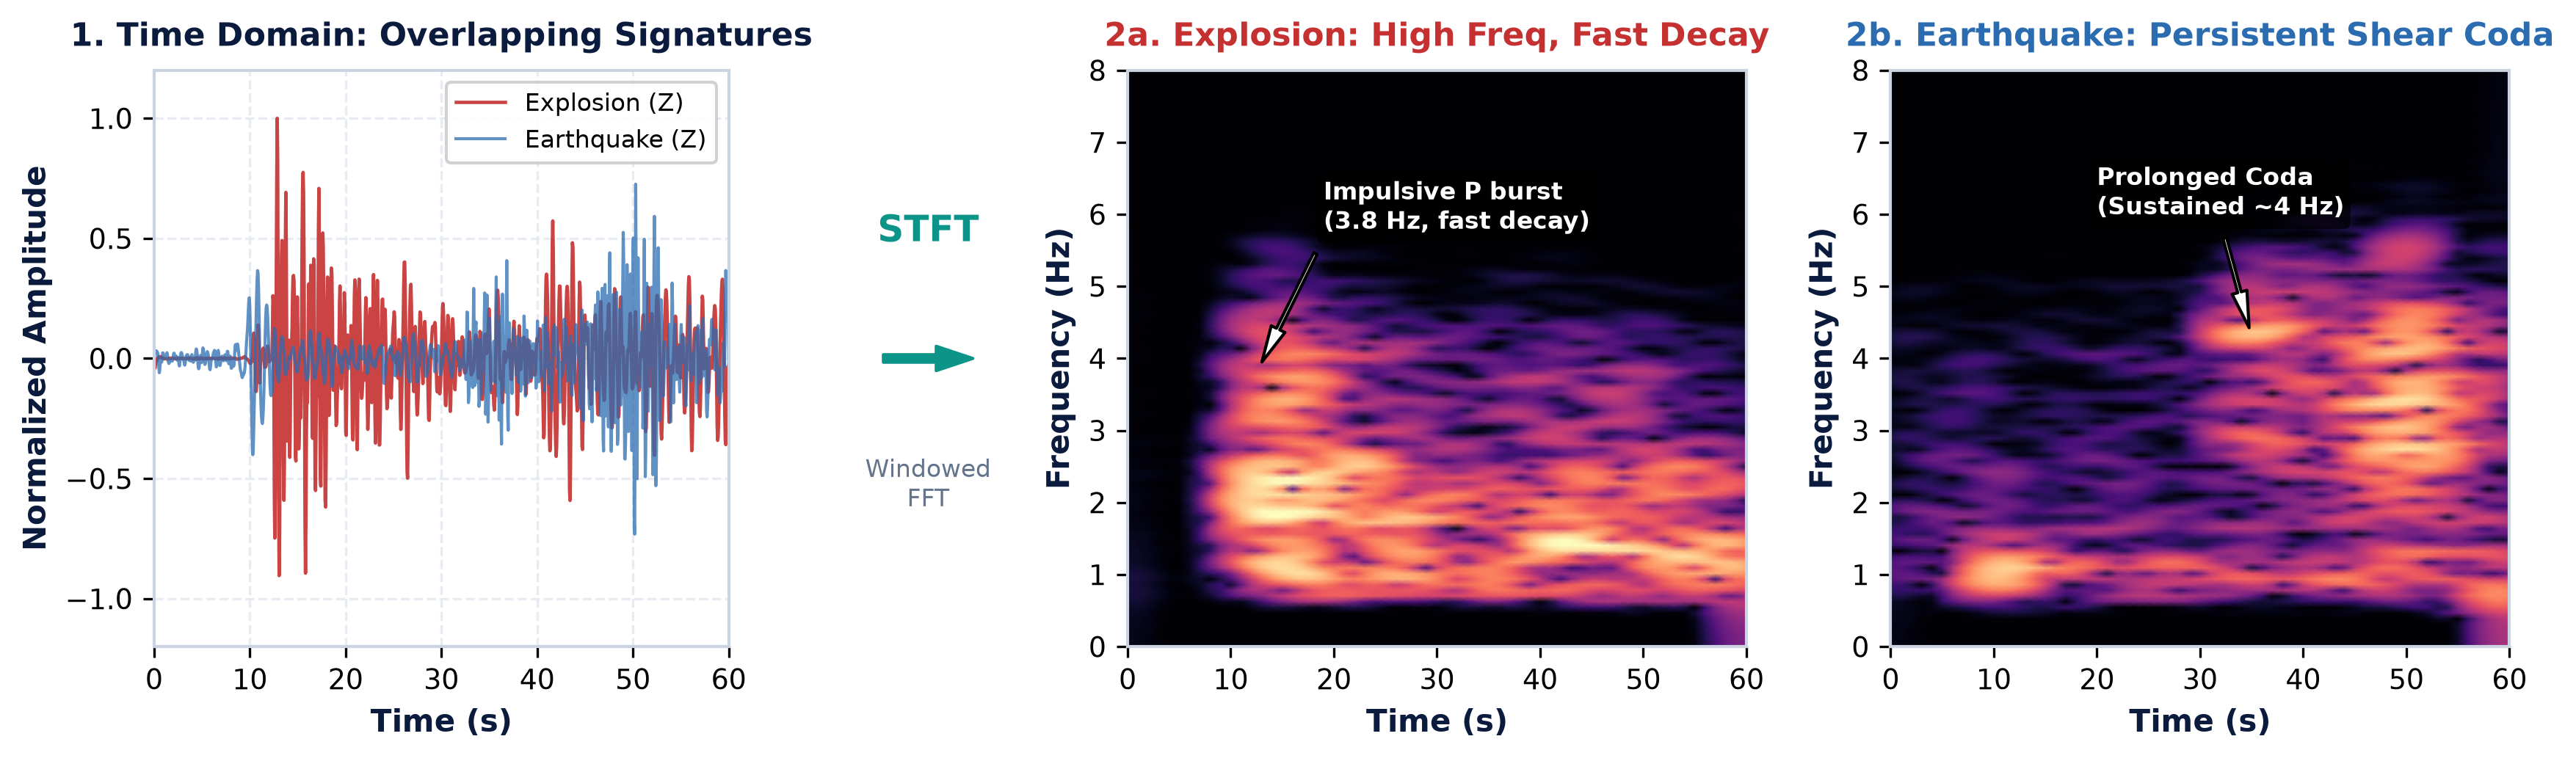
\includegraphics[width=\textwidth, height=2.5cm, keepaspectratio]{transformation_motivation.png}

  \vspace*{0.05cm}
  \small \textbf{\color{tealaccent} Workflow:} 3-Component Waveform ($3 \times 1200$) $\xrightarrow{\text{STFT}}$ 2D Spectrogram Tensors ($3 \times 128 \times 128$) $\xrightarrow{}$ Classifiers
\end{frame}

% ==============================================================================
% SLIDE 3: SECTION 1 DIVIDER
% ==============================================================================
{
\setbeamercolor{background canvas}{bg=navy}
\begin{frame}[plain]
  \vspace*{1.25cm}
  {\fontsize{13}{16}\selectfont \color{tealaccent} SECTION 01}\\[0.4em]
  {\fontsize{24}{28}\selectfont \textbf{\color{white} Signal Characteristics \& Data Curation}}\\[0.8em]
  {\fontsize{12}{15}\selectfont \color{slate} Understanding source differences and constructing a leakage-free benchmark}
\end{frame}
}

% ==============================================================================
% SLIDE 4: SEISMIC DATASETS: SOURCES, FEATURES & TEST SITES
% ==============================================================================
\begin{frame}{Seismic Datasets: Sources, Features \& Test Sites}
  \centering{\small \color{slate} Multi-station recordings, engineered feature representations, and external test sites.}\par
  \vspace*{0.08cm}

  \begin{columns}[T,onlytextwidth]
    \begin{column}{0.485\textwidth}
      \textbf{\small\color{navy} Data Sources \& Locations}
      \vspace*{0.06cm}
      \begin{itemize}\setlength{\itemsep}{0.25em}\footnotesize
        \item \textbf{Explosions (NTS, USA):} 198 recordings across 67 underground nuclear tests at Nevada Test Site (LLNL GTUNE, 1968--1992).
        \item \textbf{Earthquakes (Global/Regional):} 150 recordings across 45 tectonic events ($M_w 5.2 - 6.2$) on EarthScope GSN stations.
        \item \textbf{Unseen Test Site (DPRK):} All 6 declared North Korean underground tests (2006--2017) at Punggye-ri recorded on regional sensors (MDJ, INCN).
      \end{itemize}
    \end{column}
    \hfill
    \begin{column}{0.485\textwidth}
      \textbf{\small\color{blastred} Signal Features \& Representations}
      \vspace*{0.06cm}
      \begin{itemize}\setlength{\itemsep}{0.25em}\footnotesize
        \item \textbf{Raw Waveforms:} Synchronized 60 s window @ 20 Hz across $Z, N, E$ components ($3 \times 1,200 = 3,600$ values).
        \item \textbf{Track A (18 Physical Features):} Spectral energy ratios ($P/S$), $Z/H$ energy ratios, coda decay ($\tau$), and 3D rectilinearity.
        \item \textbf{Track B (2D Spectrogram Tensors):} $3 \times 128 \times 128$ time-frequency images extracted via STFT across components.
      \end{itemize}
    \end{column}
  \end{columns}

  \vspace*{0.12cm}
  \centering
  \footnotesize \textbf{\color{tealaccent} Evaluation Standard:} \textit{Station coordinates purged; cross-validated strictly by event ID and held out against unseen North Korean tests.}
\end{frame}

% ==============================================================================
% SLIDE 5: RAW WAVEFORMS
% ==============================================================================
\begin{frame}{Raw Waveforms: Contrasting Time-Domain Signatures}
  \vspace*{-0.1cm}
  \centering
  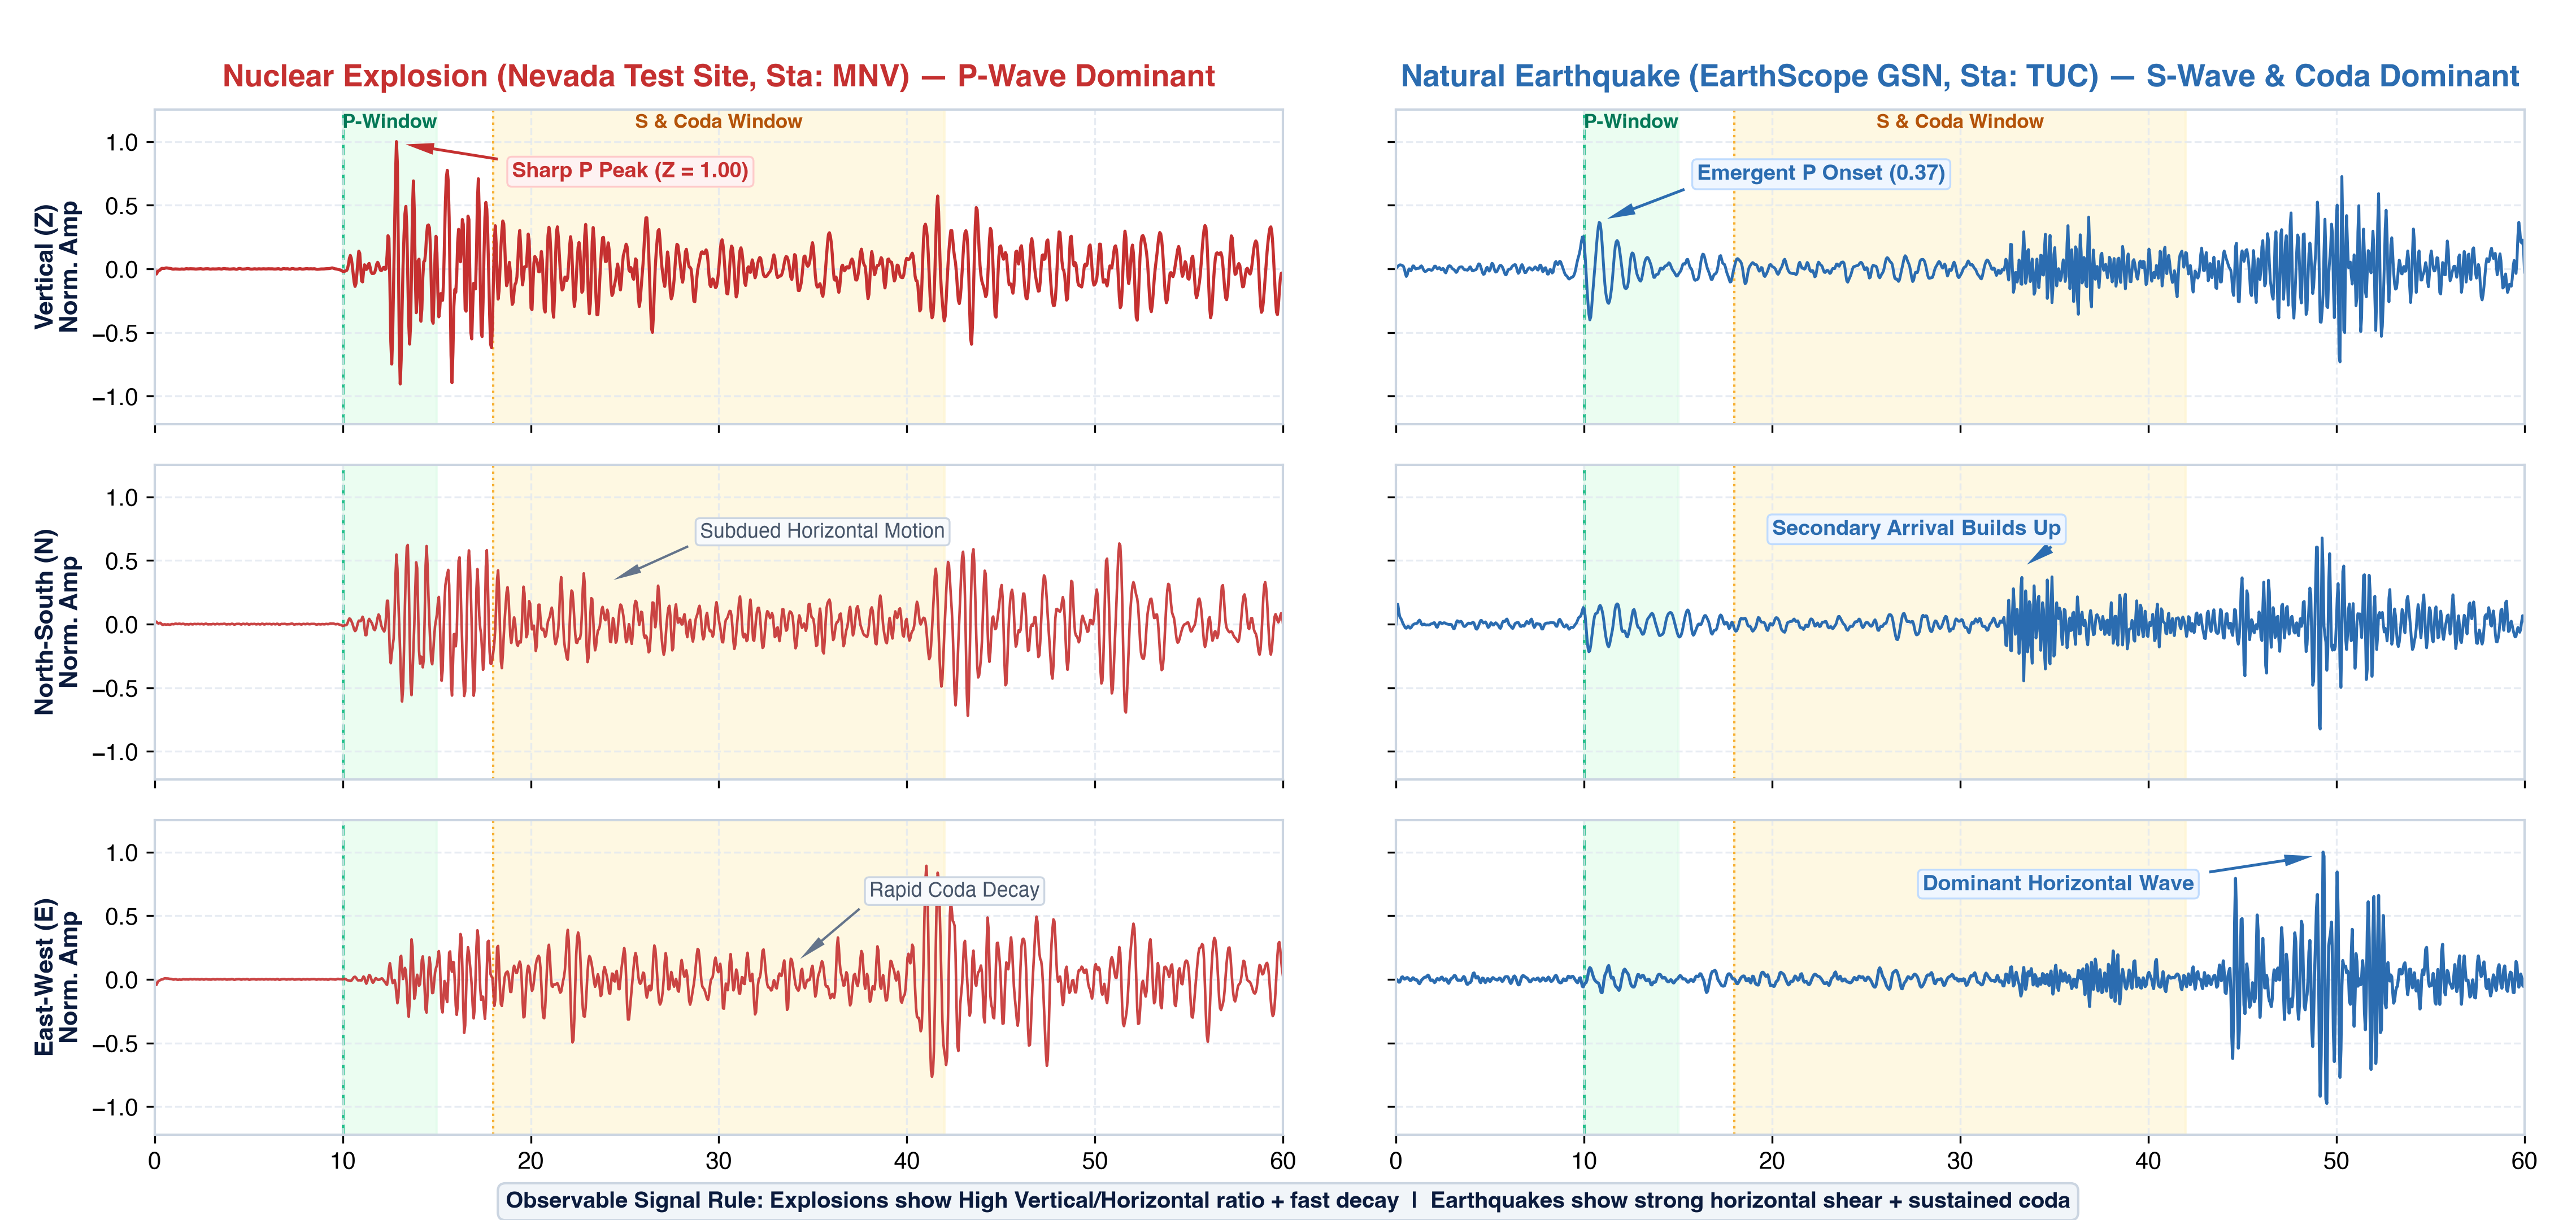
\includegraphics[width=\textwidth, height=5.35cm, keepaspectratio]{waveform_comparison.png}\\[0.15em]
  \small \color{navy}\textbf{Observed Signatures:} \textit{Explosions display sharp vertical P-waves and fast decay; earthquakes show prominent horizontal shear waves and sustained coda.}
\end{frame}

% ==============================================================================
% SLIDE 6: OBSERVABLE DIFFERENCES: EXPLOSIONS VS. EARTHQUAKES
% ==============================================================================
\begin{frame}{Observable Differences: Explosions vs. Earthquakes}
  \centering{\small \color{slate} Measurable signal properties distinguishing the two event classes across 3-component recordings.}\par
  \vspace*{0.28cm}

  \begin{columns}[T,onlytextwidth]
    \begin{column}{0.485\textwidth}
      \textbf{\color{blastred} Underground Explosion (Blast)}
      \vspace*{0.12cm}
      \begin{itemize}\setlength{\itemsep}{0.40em}\footnotesize
        \item \textbf{Impulsive Vertical Spike:} Sharp initial arrival predominantly on the vertical ($Z$) channel.
        \item \textbf{Horizontal Deficit:} Minimal motion detected on North ($N$) and East ($E$) sensors.
        \item \textbf{Early High-Frequency Burst:} Spectral energy ($>3\text{ Hz}$) concentrated at onset.
        \item \textbf{Fast Coda Decay:} Signal returns rapidly to pre-event baseline levels.
      \end{itemize}
    \end{column}
    \hfill
    \begin{column}{0.485\textwidth}
      \textbf{\color{quakeblue} Natural Earthquake (Tectonic Event)}
      \vspace*{0.12cm}
      \begin{itemize}\setlength{\itemsep}{0.40em}\footnotesize
        \item \textbf{Emergent Onset:} Amplitude builds gradually over several seconds.
        \item \textbf{Intense Horizontal Shaking:} Dominant motion on North ($N$) and East ($E$) sensors.
        \item \textbf{Persistent Low Frequencies:} Spectral power concentrated in low-to-mid bands ($<3\text{ Hz}$).
        \item \textbf{Prolonged Coda Duration:} Reverberating late-phase waves continue for 40+ seconds.
      \end{itemize}
    \end{column}
  \end{columns}

  \vspace*{0.32cm}
  \centering
  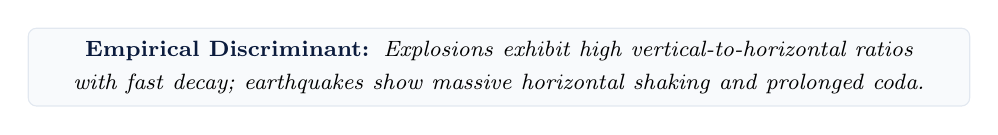
\begin{tikzpicture}
    \node[rectangle, draw=bordergray, fill=lightbg, rounded corners=3pt, inner sep=4.5pt, text width=0.96\textwidth, align=center] {
      \footnotesize \textbf{\color{navy} Empirical Discriminant:} \textit{Explosions exhibit high vertical-to-horizontal ratios with fast decay; earthquakes show massive horizontal shaking and prolonged coda.}
    };
  \end{tikzpicture}
\end{frame}

% ==============================================================================
% SLIDE 7: SECTION 2 DIVIDER
% ==============================================================================
{
\setbeamercolor{background canvas}{bg=navy}
\begin{frame}[plain]
  \vspace*{1.25cm}
  {\fontsize{13}{16}\selectfont \color{tealaccent} SECTION 02}\\[0.4em]
  {\fontsize{24}{28}\selectfont \textbf{\color{white} Classification Methods}}\\[0.8em]
  {\fontsize{12}{15}\selectfont \color{slate} Formulations, loss functions, and regularization across classical ML and deep learning}
\end{frame}
}

% ==============================================================================
% SLIDE 8: TWO APPROACHES TO CLASSIFICATION
% ==============================================================================
\begin{frame}{Two Approaches to Classification}
  \vspace*{0.1cm}
  \centering
  \resizebox{\textwidth}{!}{
    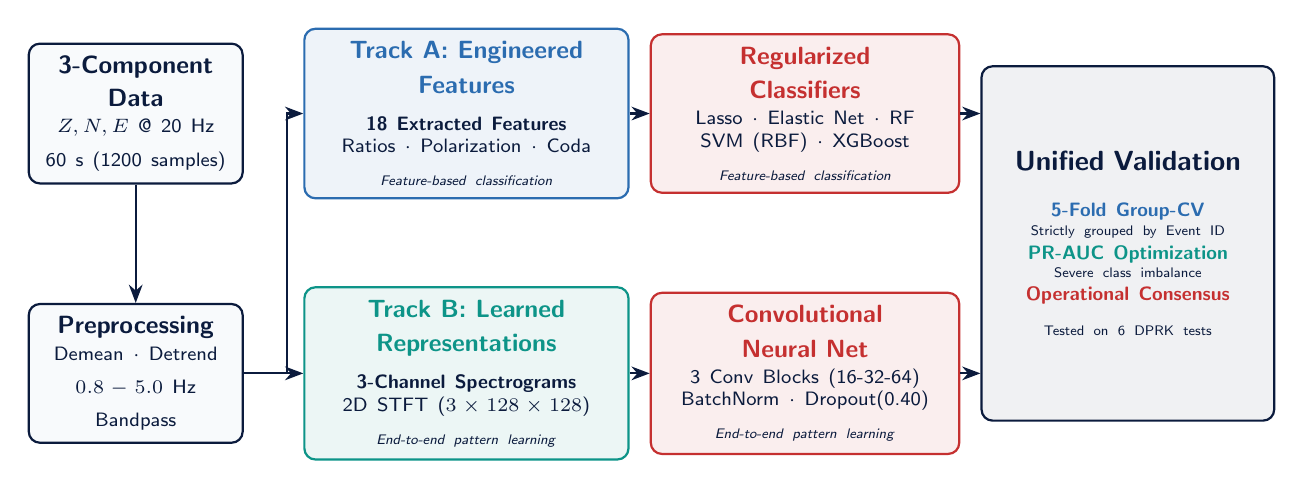
\begin{tikzpicture}[
      font=\sffamily,
      box/.style={rectangle, draw=bordergray, thick, rounded corners=4pt, inner sep=4.5pt, align=center},
      inpbox/.style={box, draw=navy, fill=lightbg, text=navy},
      trackA/.style={box, draw=quakeblue, fill=quakeblue!8, text=navy},
      trackB/.style={box, draw=tealaccent, fill=tealaccent!8, text=navy},
      modelbox/.style={box, draw=blastred, fill=blastred!8, text=navy},
      evalbox/.style={box, draw=navy, fill=navy!6, text=navy},
      arr/.style={-{Stealth[scale=1.0]}, draw=navy, thick}
    ]

      % Column 1: Input & Preprocessing
      \node[inpbox, text width=2.4cm, minimum height=1.35cm] (raw) at (0, 1.65) {
        \textbf{\small 3-Component Data}\\[0.15em]
        \scriptsize $Z, N, E$ @ 20 Hz\\
        60 s (1200 samples)
      };

      \node[inpbox, text width=2.4cm, minimum height=1.35cm] (prep) at (0, -1.65) {
        \textbf{\small Preprocessing}\\[0.15em]
        \scriptsize Demean $\cdot$ Detrend\\
        $0.8 - 5.0\text{ Hz}$ Bandpass
      };

      % Column 2: Representations
      \node[trackA, text width=3.8cm, minimum height=1.45cm] (feat) at (4.2, 1.65) {
        \textbf{\small\color{quakeblue} Track A: Engineered}\\[0.05em]
        \textbf{\small\color{quakeblue} Features}\\[0.15em]
        \textbf{\scriptsize 18 Extracted Features}\\
        \scriptsize Ratios $\cdot$ Polarization $\cdot$ Coda\\
        \textit{\tiny Feature-based classification}
      };

      \node[trackB, text width=3.8cm, minimum height=1.45cm] (stft) at (4.2, -1.65) {
        \textbf{\small\color{tealaccent} Track B: Learned}\\[0.05em]
        \textbf{\small\color{tealaccent} Representations}\\[0.15em]
        \textbf{\scriptsize 3-Channel Spectrograms}\\
        \scriptsize 2D STFT ($3 \times 128 \times 128$)\\
        \textit{\tiny End-to-end pattern learning}
      };

      % Column 3: Models
      \node[modelbox, text width=3.6cm, minimum height=1.45cm] (ml) at (8.5, 1.65) {
        \textbf{\small\color{blastred} Regularized}\\[0.05em]
        \textbf{\small\color{blastred} Classifiers}\\[0.15em]
        \scriptsize Lasso $\cdot$ Elastic Net $\cdot$ RF\\
        \scriptsize SVM (RBF) $\cdot$ XGBoost\\
        \textit{\tiny Feature-based classification}
      };

      \node[modelbox, text width=3.6cm, minimum height=1.45cm] (cnn) at (8.5, -1.65) {
        \textbf{\small\color{blastred} Convolutional}\\[0.05em]
        \textbf{\small\color{blastred} Neural Net}\\[0.15em]
        \scriptsize 3 Conv Blocks (16-32-64)\\
        \scriptsize BatchNorm $\cdot$ Dropout(0.40)\\
        \textit{\tiny End-to-end pattern learning}
      };

      % Column 4: Unified Validation & Operational Decision
      \node[evalbox, text width=3.4cm, minimum height=4.5cm] (eval) at (12.6, 0) {
        \textbf{\normalsize\color{navy} Unified Validation}\\[0.45em]
        \textbf{\scriptsize\color{quakeblue} 5-Fold Group-CV}\\[0.1em]
        \tiny Strictly grouped by Event ID\\[0.45em]
        \textbf{\scriptsize\color{tealaccent} PR-AUC Optimization}\\[0.1em]
        \tiny Severe class imbalance\\[0.45em]
        \textbf{\scriptsize\color{blastred} Operational Consensus}\\[0.1em]
        \tiny Tested on 6 DPRK tests
      };

      % Connecting Arrows
      \draw[arr] (raw) -- (prep);
      \draw[arr] (prep.east) -- ++(0.55, 0) |- (feat.west);
      \draw[arr] (prep.east) -- ++(0.55, 0) |- (stft.west);
      \draw[arr] (feat) -- (ml);
      \draw[arr] (stft) -- (cnn);
      \draw[arr] (ml.east) -- (eval.west |- ml.east);
      \draw[arr] (cnn.east) -- (eval.west |- cnn.east);

    \end{tikzpicture}
  }

  \vspace*{0.25cm}
  \footnotesize \color{navy}\textbf{Benchmarking Objective:} \textit{Compare manual feature construction against automatic representation learning under identical, strictly event-grouped cross-validation splits.}
\end{frame}

% ==============================================================================
% SLIDE 9: TRACK A - LASSO LOGISTIC REGRESSION (L1)
% ==============================================================================
\begin{frame}{Track A: Lasso Logistic Regression ($L_1$ Regularization)}
  \vspace*{0.05cm}

  \centering
  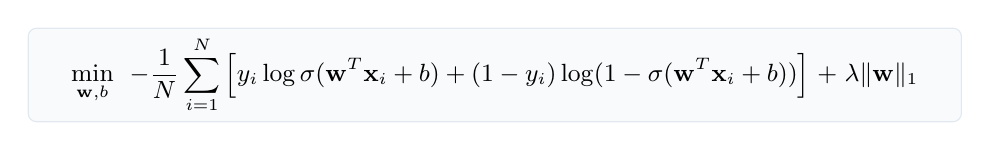
\begin{tikzpicture}
    \node[rectangle, draw=bordergray, fill=lightbg, rounded corners=3pt, inner sep=3pt, text width=0.96\textwidth, align=center] {
      \small $\displaystyle \min_{\mathbf{w}, b} \; -\frac{1}{N}\sum_{i=1}^N \left[ y_i \log \sigma(\mathbf{w}^T \mathbf{x}_i + b) + (1 - y_i) \log(1 - \sigma(\mathbf{w}^T \mathbf{x}_i + b)) \right] + \lambda \|\mathbf{w}\|_1$
    };
  \end{tikzpicture}

  \vspace*{0.12cm}
  \begin{columns}[T,onlytextwidth]
    \begin{column}{0.48\textwidth}
      \textbf{\small\color{navy} $L_1$ Sparsity Mechanism}
      \vspace*{0.08cm}
      \begin{itemize}\setlength{\itemsep}{0.25em}\footnotesize
        \item \textbf{Feature Zeroing:} $L_1$ penalty ($\|\mathbf{w}\|_1 = \sum |w_j|$) drives redundant feature weights strictly to zero.
        \item \textbf{Physical Selection:} Retains cross-phase spectral ratios while discarding noisy kurtosis metrics.
        \item \textbf{Linear Baseline:} Provides clean, interpretable log-odds ratios for source discrimination.
      \end{itemize}
    \end{column}
    \hfill
    \begin{column}{0.48\textwidth}
      \textbf{\small\color{blastred} Tuning \& Performance}
      \vspace*{0.08cm}
      \begin{itemize}\setlength{\itemsep}{0.25em}\footnotesize
        \item \textbf{Optimal Parameter:} $C = \frac{1}{\lambda} = 2.0$ (SAGA solver).
        \item \textbf{5-Fold CV Results:}
          \begin{itemize}\scriptsize
            \item Accuracy: \textbf{95.98\%} $\quad$ Precision: \textbf{98.36\%}
            \item Recall: \textbf{92.58\%} $\quad$ PR-AUC: \textbf{0.9943}
          \end{itemize}
        \item \textbf{Role:} Fast, highly interpretable linear reference.
      \end{itemize}
    \end{column}
  \end{columns}
\end{frame}

% ==============================================================================
% SLIDE 10: TRACK A - ELASTIC NET LOGISTIC REGRESSION (L1 + L2)
% ==============================================================================
\begin{frame}{Track A: Elastic Net Logistic Regression ($L_1 + L_2$ Penalty)}
  \vspace*{0.05cm}

  \centering
  
\begin{tikzpicture}
    \node[rectangle, draw=bordergray, fill=lightbg, rounded corners=3pt, inner sep=3pt, text width=0.96\textwidth, align=center] {
      \small $\displaystyle \min_{\mathbf{w}, b} \; \mathcal{L}_{\text{log}}(\mathbf{w}, b) + \lambda \left[ \alpha \|\mathbf{w}\|_1 + \frac{1-\alpha}{2} \|\mathbf{w}\|_2^2 \right], \quad \alpha \in [0, 1] \text{ (\texttt{l1\_ratio})}$
    };
  \end{tikzpicture}

  \vspace*{0.12cm}
  \begin{columns}[T,onlytextwidth]
    \begin{column}{0.48\textwidth}
      \textbf{\small\color{navy} Grouping \& Collinearity}
      \vspace*{0.08cm}
      \begin{itemize}\setlength{\itemsep}{0.25em}\footnotesize
        \item \textbf{Overcomes Lasso Limit:} Retains correlated features jointly instead of dropping one at random.
        \item \textbf{Cross-Channel Grouping:} Selects complementary vertical ($Z$) and horizontal ($H$) features together.
        \item \textbf{Numerical Stability:} Strictly convex $L_2$ term stabilizes optimization under collinear ratios.
      \end{itemize}
    \end{column}
    \hfill
    \begin{column}{0.48\textwidth}
      \textbf{\small\color{blastred} Tuning \& Performance}
      \vspace*{0.08cm}
      \begin{itemize}\setlength{\itemsep}{0.25em}\footnotesize
        \item \textbf{Optimal Parameters:} $C = 2.0$, $\alpha = 0.80$ ($80\%$ $L_1$, $20\%$ $L_2$).
        \item \textbf{5-Fold CV Results:}
          \begin{itemize}\scriptsize
            \item Accuracy: \textbf{96.27\%} $\quad$ Precision: \textbf{98.40\%}
            \item Recall: \textbf{94.53\%} $\quad$ PR-AUC: \textbf{0.9940}
          \end{itemize}
        \item \textbf{Gain over Lasso:} Improves recall by \textbf{+1.95\%} by preserving multi-channel dynamics.
      \end{itemize}
    \end{column}
  \end{columns}
\end{frame}

% ==============================================================================
% SLIDE 11: TRACK A - RANDOM FOREST CLASSIFIER
% ==============================================================================
\begin{frame}{Track A: Random Forest Classifier (Bagging Ensemble)}
  \vspace*{0.05cm}

  \centering
  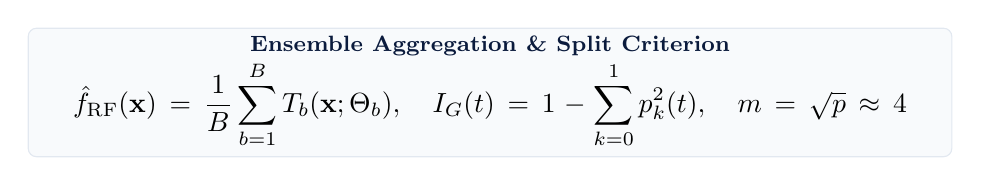
\begin{tikzpicture}
    \node[rectangle, draw=bordergray, fill=lightbg, rounded corners=3pt, inner sep=3pt, text width=0.95\textwidth, align=center] {
      \textbf{\footnotesize\color{navy} Ensemble Aggregation \& Split Criterion}\\[0.1em]
      $\displaystyle \hat{f}_{\text{RF}}(\mathbf{x}) = \frac{1}{B}\sum_{b=1}^B T_b(\mathbf{x}; \Theta_b), \quad I_G(t) = 1 - \sum_{k=0}^1 p_k^2(t), \quad m = \sqrt{p} \approx 4$
    };
  \end{tikzpicture}

  \vspace*{0.12cm}
  \begin{columns}[T,onlytextwidth]
    \begin{column}{0.48\textwidth}
      \textbf{\small\color{navy} Ensemble Mechanism}
      \vspace*{0.08cm}
      \begin{itemize}\setlength{\itemsep}{0.25em}\footnotesize
        \item \textbf{Bootstrap Aggregation:} Averages $B = 200$ de-correlated trees to minimize model variance.
        \item \textbf{Subspace Sampling:} Evaluates $m \approx 4$ random features per split, preventing single-feature dominance.
        \item \textbf{Non-Linear Thresholds:} Captures complex wave-property interactions without distribution assumptions.
      \end{itemize}
    \end{column}
    \hfill
    \begin{column}{0.48\textwidth}
      \textbf{\small\color{blastred} Tuning \& Performance}
      \vspace*{0.08cm}
      \begin{itemize}\setlength{\itemsep}{0.25em}\footnotesize
        \item \textbf{Configuration:} $B = 200$ trees, $\text{max\_depth} = 8$.
        \item \textbf{5-Fold CV Results:}
          \begin{itemize}\scriptsize
            \item Accuracy: \textbf{96.26\%} $\quad$ Precision: \textbf{97.39\%}
            \item Recall: \textbf{95.53\%} $\quad$ PR-AUC: \textbf{0.9936}
          \end{itemize}
        \item \textbf{Robustness:} Tree consensus resists sensor dropouts and noise spikes.
      \end{itemize}
    \end{column}
  \end{columns}
\end{frame}

% ==============================================================================
% SLIDE 12: TRACK A - SUPPORT VECTOR MACHINE (RBF KERNEL)
% ==============================================================================
\begin{frame}{Track A: Support Vector Machine (RBF Kernel)}
  \vspace*{0.05cm}

  \centering
  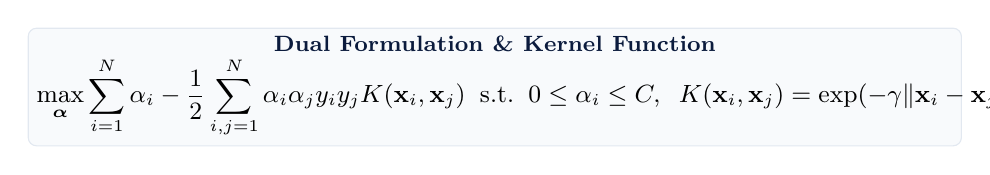
\begin{tikzpicture}
    \node[rectangle, draw=bordergray, fill=lightbg, rounded corners=3pt, inner sep=3pt, text width=0.96\textwidth, align=center] {
      \textbf{\footnotesize\color{navy} Dual Formulation \& Kernel Function}\\[0.1em]
      \mbox{\small $\displaystyle \max_{\boldsymbol{\alpha}} \sum_{i=1}^N \alpha_i - \frac{1}{2}\sum_{i,j=1}^N \alpha_i \alpha_j y_i y_j K(\mathbf{x}_i, \mathbf{x}_j) \;\;\text{s.t.}\;\; 0 \le \alpha_i \le C, \;\; K(\mathbf{x}_i, \mathbf{x}_j) = \exp(-\gamma \|\mathbf{x}_i - \mathbf{x}_j\|^2)$}
    };
  \end{tikzpicture}

  \vspace*{0.12cm}
  \begin{columns}[T,onlytextwidth]
    \begin{column}{0.48\textwidth}
      \textbf{\small\color{navy} Kernel Margin Separation}
      \vspace*{0.08cm}
      \begin{itemize}\setlength{\itemsep}{0.25em}\footnotesize
        \item \textbf{RBF Projection:} Projects 18D features into Hilbert space for non-linear boundary separation.
        \item \textbf{Support Vector Sparsity:} Decision boundary depends strictly on margin-defining boundary points.
        \item \textbf{Calibrated Confidence:} Platt scaling converts margin distances into calibrated probability scores.
      \end{itemize}
    \end{column}
    \hfill
    \begin{column}{0.48\textwidth}
      \textbf{\small\color{blastred} Tuning \& Performance}
      \vspace*{0.08cm}
      \begin{itemize}\setlength{\itemsep}{0.25em}\footnotesize
        \item \textbf{Optimal Parameters:} Penalty $C = 20.0$, bandwidth $\gamma = 0.01$.
        \item \textbf{5-Fold CV Results:}
          \begin{itemize}\scriptsize
            \item Accuracy: \textbf{\color{blastred} 97.13\%} (Top Tabular Model)
            \item Precision: \textbf{97.45\%} $\quad$ Recall: \textbf{97.05\%}
            \item PR-AUC: \textbf{\color{blastred} 0.9973}
          \end{itemize}
        \item \textbf{Key Takeaway:} Best classical ML performer, rivaling deep learning accuracy.
      \end{itemize}
    \end{column}
  \end{columns}
\end{frame}

% ==============================================================================
% SLIDE 13: TRACK A - XGBOOST CLASSIFIER
% ==============================================================================
\begin{frame}{Track A: XGBoost Classifier (Gradient Boosted Trees)}
  \vspace*{0.05cm}

  \centering
  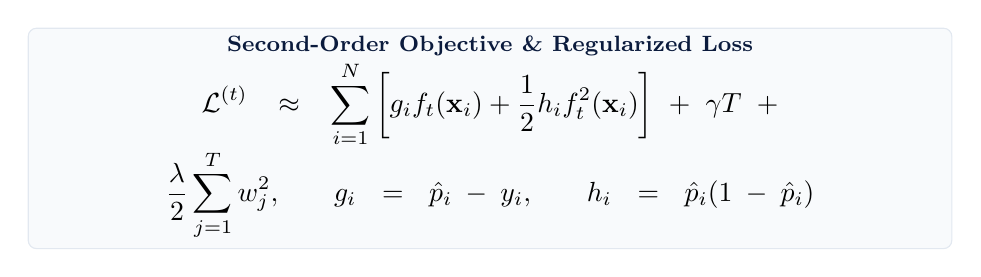
\begin{tikzpicture}
    \node[rectangle, draw=bordergray, fill=lightbg, rounded corners=3pt, inner sep=3pt, text width=0.95\textwidth, align=center] {
      \textbf{\footnotesize\color{navy} Second-Order Objective \& Regularized Loss}\\[0.1em]
      $\displaystyle \mathcal{L}^{(t)} \approx \sum_{i=1}^N \left[ g_i f_t(\mathbf{x}_i) + \frac{1}{2} h_i f_t^2(\mathbf{x}_i) \right] + \gamma T + \frac{\lambda}{2}\sum_{j=1}^T w_j^2, \;\; g_i = \hat{p}_i - y_i, \;\; h_i = \hat{p}_i(1 - \hat{p}_i)$
    };
  \end{tikzpicture}

  \vspace*{0.12cm}
  \begin{columns}[T,onlytextwidth]
    \begin{column}{0.48\textwidth}
      \textbf{\small\color{navy} Gradient Tree Boosting}
      \vspace*{0.08cm}
      \begin{itemize}\setlength{\itemsep}{0.25em}\footnotesize
        \item \textbf{Second-Order Curvature:} Uses exact gradients ($g_i$) and Hessians ($h_i$) for rapid, precise descent.
        \item \textbf{Complexity Control:} Penalizes total leaves ($\gamma T$) and leaf weights ($\lambda \|w\|^2$) to prevent overfitting.
        \item \textbf{Shrinkage \& Subsampling:} Step size $\eta = 0.05$ with $80\%$ subsampling ensures gradual, robust learning.
      \end{itemize}
    \end{column}
    \hfill
    \begin{column}{0.48\textwidth}
      \textbf{\small\color{blastred} Tuning \& Performance}
      \vspace*{0.08cm}
      \begin{itemize}\setlength{\itemsep}{0.25em}\footnotesize
        \item \textbf{Configuration:} 200 trees, $\text{depth} = 4$, $\eta = 0.05$.
        \item \textbf{5-Fold CV Results:}
          \begin{itemize}\scriptsize
            \item Accuracy: \textbf{96.55\%} $\quad$ Precision: \textbf{97.89\%}
            \item Recall: \textbf{95.53\%} $\quad$ PR-AUC: \textbf{0.9954}
          \end{itemize}
        \item \textbf{Physical Feature Gain:} Horizontal spectral spread (\texttt{spec\_spread\_h}) leads with **48.1\%** gain.
      \end{itemize}
    \end{column}
  \end{columns}
\end{frame}

% ==============================================================================
% SLIDE 14: TRACK B - LEARNING PATTERNS FROM SPECTROGRAMS
% ==============================================================================
\begin{frame}{Track B: Learning Discriminative Patterns from Spectrograms}
  \vspace*{0.05cm}
  \centering
  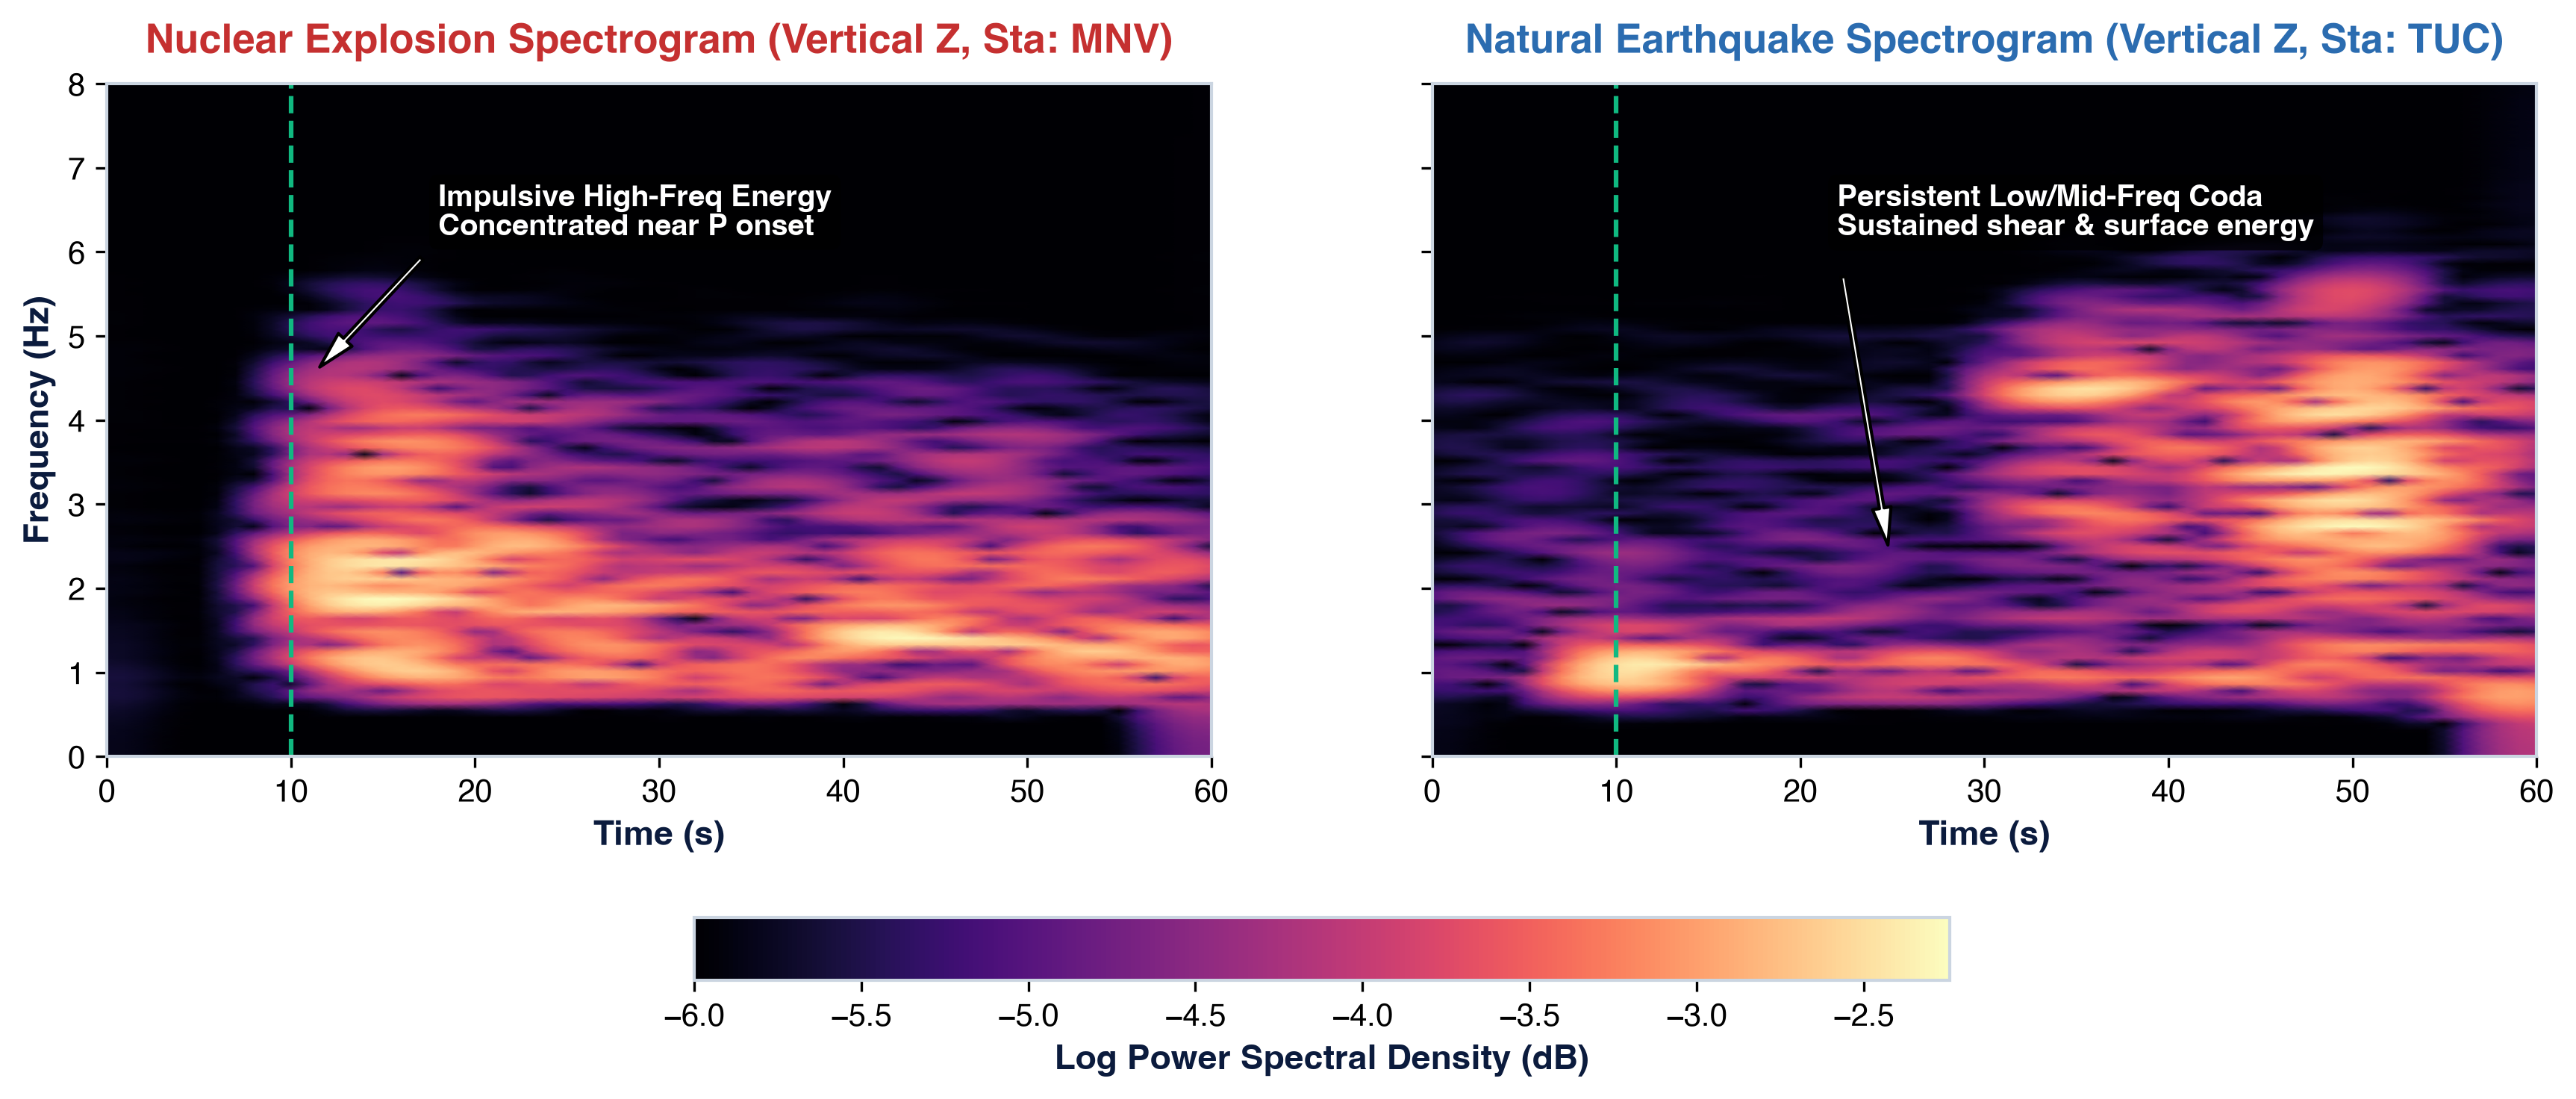
\includegraphics[height=4.75cm, keepaspectratio]{spectrogram_comparison.png}

  \vspace*{0.12cm}
  \begin{columns}[T,onlytextwidth]
    \begin{column}{0.31\textwidth}
      \centering
      \textbf{\color{blastred}\small Explosions}\\[0.1em]
      \scriptsize High frequencies concentrated at arrival; rapid temporal decay.
    \end{column}
    \hfill
    \begin{column}{0.31\textwidth}
      \centering
      \textbf{\color{navy}\small Earthquakes}\\[0.1em]
      \scriptsize Prolonged low/mid-frequency energy spanning the entire 60 s record.
    \end{column}
    \hfill
    \begin{column}{0.31\textwidth}
      \centering
      \textbf{\color{tealaccent}\small CNN Pattern Learning}\\[0.1em]
      \scriptsize Learns these 2D patterns directly without manually specified rules.
    \end{column}
  \end{columns}
\end{frame}

% ==============================================================================
% SLIDE 15: TRACK B - 3-CHANNEL 2D CNN ARCHITECTURE
% ==============================================================================
\begin{frame}{Track B: 3-Channel 2D Convolutional Neural Network (CNN)}
  \vspace*{0.05cm}

  \centering
  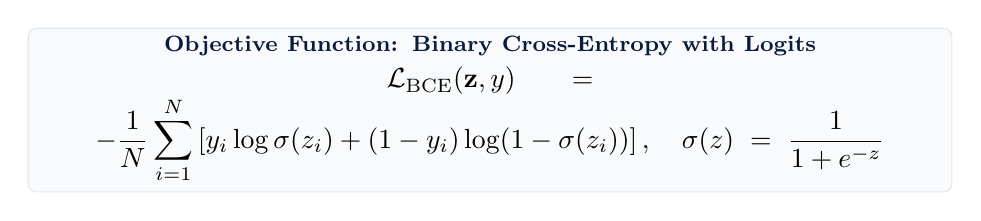
\begin{tikzpicture}
    \node[rectangle, draw=bordergray, fill=lightbg, rounded corners=3pt, inner sep=3pt, text width=0.95\textwidth, align=center] {
      \textbf{\footnotesize\color{navy} Objective Function: Binary Cross-Entropy with Logits}\\[0.1em]
      $\displaystyle \mathcal{L}_{\text{BCE}}(\mathbf{z}, y) = -\frac{1}{N}\sum_{i=1}^N \left[ y_i \log \sigma(z_i) + (1 - y_i) \log(1 - \sigma(z_i)) \right], \quad \sigma(z) = \frac{1}{1 + e^{-z}}$
    };
  \end{tikzpicture}

  \vspace*{0.12cm}
  \begin{columns}[T,onlytextwidth]
    \begin{column}{0.48\textwidth}
      \textbf{\small\color{tealaccent} CNN Architecture}
      \vspace*{0.08cm}
      \begin{itemize}\setlength{\itemsep}{0.25em}\footnotesize
        \item \textbf{Input Tensor:} $3 \times 128 \times 128$ ($Z, N, E$ spectrograms).
        \item \textbf{4 Conv Blocks:} $3 \to 32 \to 64 \to 128 \to 128$ filters with BatchNorm, ReLU, and MaxPool.
        \item \textbf{Head:} Global pooling $\to$ Dense(128) with Dropout(0.4) $\to$ single output logit.
      \end{itemize}
    \end{column}
    \hfill
    \begin{column}{0.48\textwidth}
      \textbf{\small\color{blastred} Training \& Performance}
      \vspace*{0.08cm}
      \begin{itemize}\setlength{\itemsep}{0.25em}\footnotesize
        \item \textbf{Training:} AdamW ($\text{lr} = 10^{-3}$, decay $= 10^{-2}$), Cosine Annealing.
        \item \textbf{5-Fold CV Results:}
          \begin{itemize}\scriptsize
            \item Accuracy: \textbf{\color{blastred} 97.98\%} (Rank \#1 Overall)
            \item Precision: \textbf{\color{blastred} 99.01\%} $\quad$ Recall: \textbf{97.54\%}
            \item PR-AUC: \textbf{\color{blastred} 0.9976}
          \end{itemize}
        \item \textbf{Advantage:} Directly learns 2D spectral transitions without manual feature engineering.
      \end{itemize}
    \end{column}
  \end{columns}
\end{frame}

% ==============================================================================
% SLIDE 11: SECTION 3 DIVIDER
% ==============================================================================
{
\setbeamercolor{background canvas}{bg=navy}
\begin{frame}[plain]
  \vspace*{1.25cm}
  {\fontsize{13}{16}\selectfont \color{tealaccent} SECTION 03}\\[0.4em]
  {\fontsize{24}{28}\selectfont \textbf{\color{white} Benchmark Results \& Feature Importance}}\\[0.8em]
  {\fontsize{12}{15}\selectfont \color{slate} Model leaderboard, precision-recall trade-offs, and signal discriminants}
\end{frame}
}

% ==============================================================================
% SLIDE 12: MODEL LEADERBOARD (Clean & Accessible)
% ==============================================================================
\begin{frame}{Model Leaderboard: 3-Channel CNN Outperforms Classical ML}
  \centering{\normalsize \color{slate} 5-Fold Event-Grouped Cross-Validation (Evaluated with zero geographic data leakage)}\par
  \vspace*{0.25cm}

  \centering
  \resizebox{\textwidth}{!}{
  \renewcommand{\arraystretch}{1.25}
  \begin{tabular}{llcccc}
    \toprule
    \textbf{Rank} & \textbf{Model Family} & \textbf{Accuracy (\%)} & \textbf{Precision (\%)} & \textbf{Recall (\%)} & \textbf{PR-AUC} \\
    \midrule
    \textbf{1} & \textbf{3-Channel 2D CNN (Spectrograms)} & \textbf{97.98} & \textbf{99.01} & \textbf{97.54} & \textbf{0.9976} \\
    2 & Support Vector Machine (RBF Kernel) & 97.13 & 97.45 & 97.05 & 0.9973 \\
    3 & XGBoost (Gradient Boosted Trees) & 96.55 & 97.89 & 95.53 & 0.9954 \\
    4 & Elastic Net Logistic Regression & 96.27 & 98.40 & 94.53 & 0.9940 \\
    5 & Random Forest & 96.26 & 97.39 & 95.53 & 0.9936 \\
    6 & Lasso Logistic Regression ($L_1$) & 95.98 & 98.36 & 92.58 & 0.9943 \\
    \bottomrule
  \end{tabular}
  }

  \vspace*{0.35cm}
  \begin{columns}[T,onlytextwidth]
    \begin{column}{0.485\textwidth}
      \footnotesize \textbf{\color{tealaccent} CNN Representation Advantage:} Learning directly from 2D spectrograms captures joint time-frequency patterns that summary features miss, leading across all metrics.
    \end{column}
    \hfill
    \begin{column}{0.485\textwidth}
      \footnotesize \textbf{\color{navy} Strong Tabular Baselines:} Non-linear SVM and tree models achieve $>96\%$ accuracy, proving that engineered energy ratios and frequency metrics capture substantial signal.
    \end{column}
  \end{columns}
\end{frame}

% ==============================================================================
% SLIDE 13: BENCHMARK VISUALIZATION
% ==============================================================================
\begin{frame}{Performance Benchmark: Multi-Metric Model Comparison}
  \vspace*{-0.1cm}
  \centering
  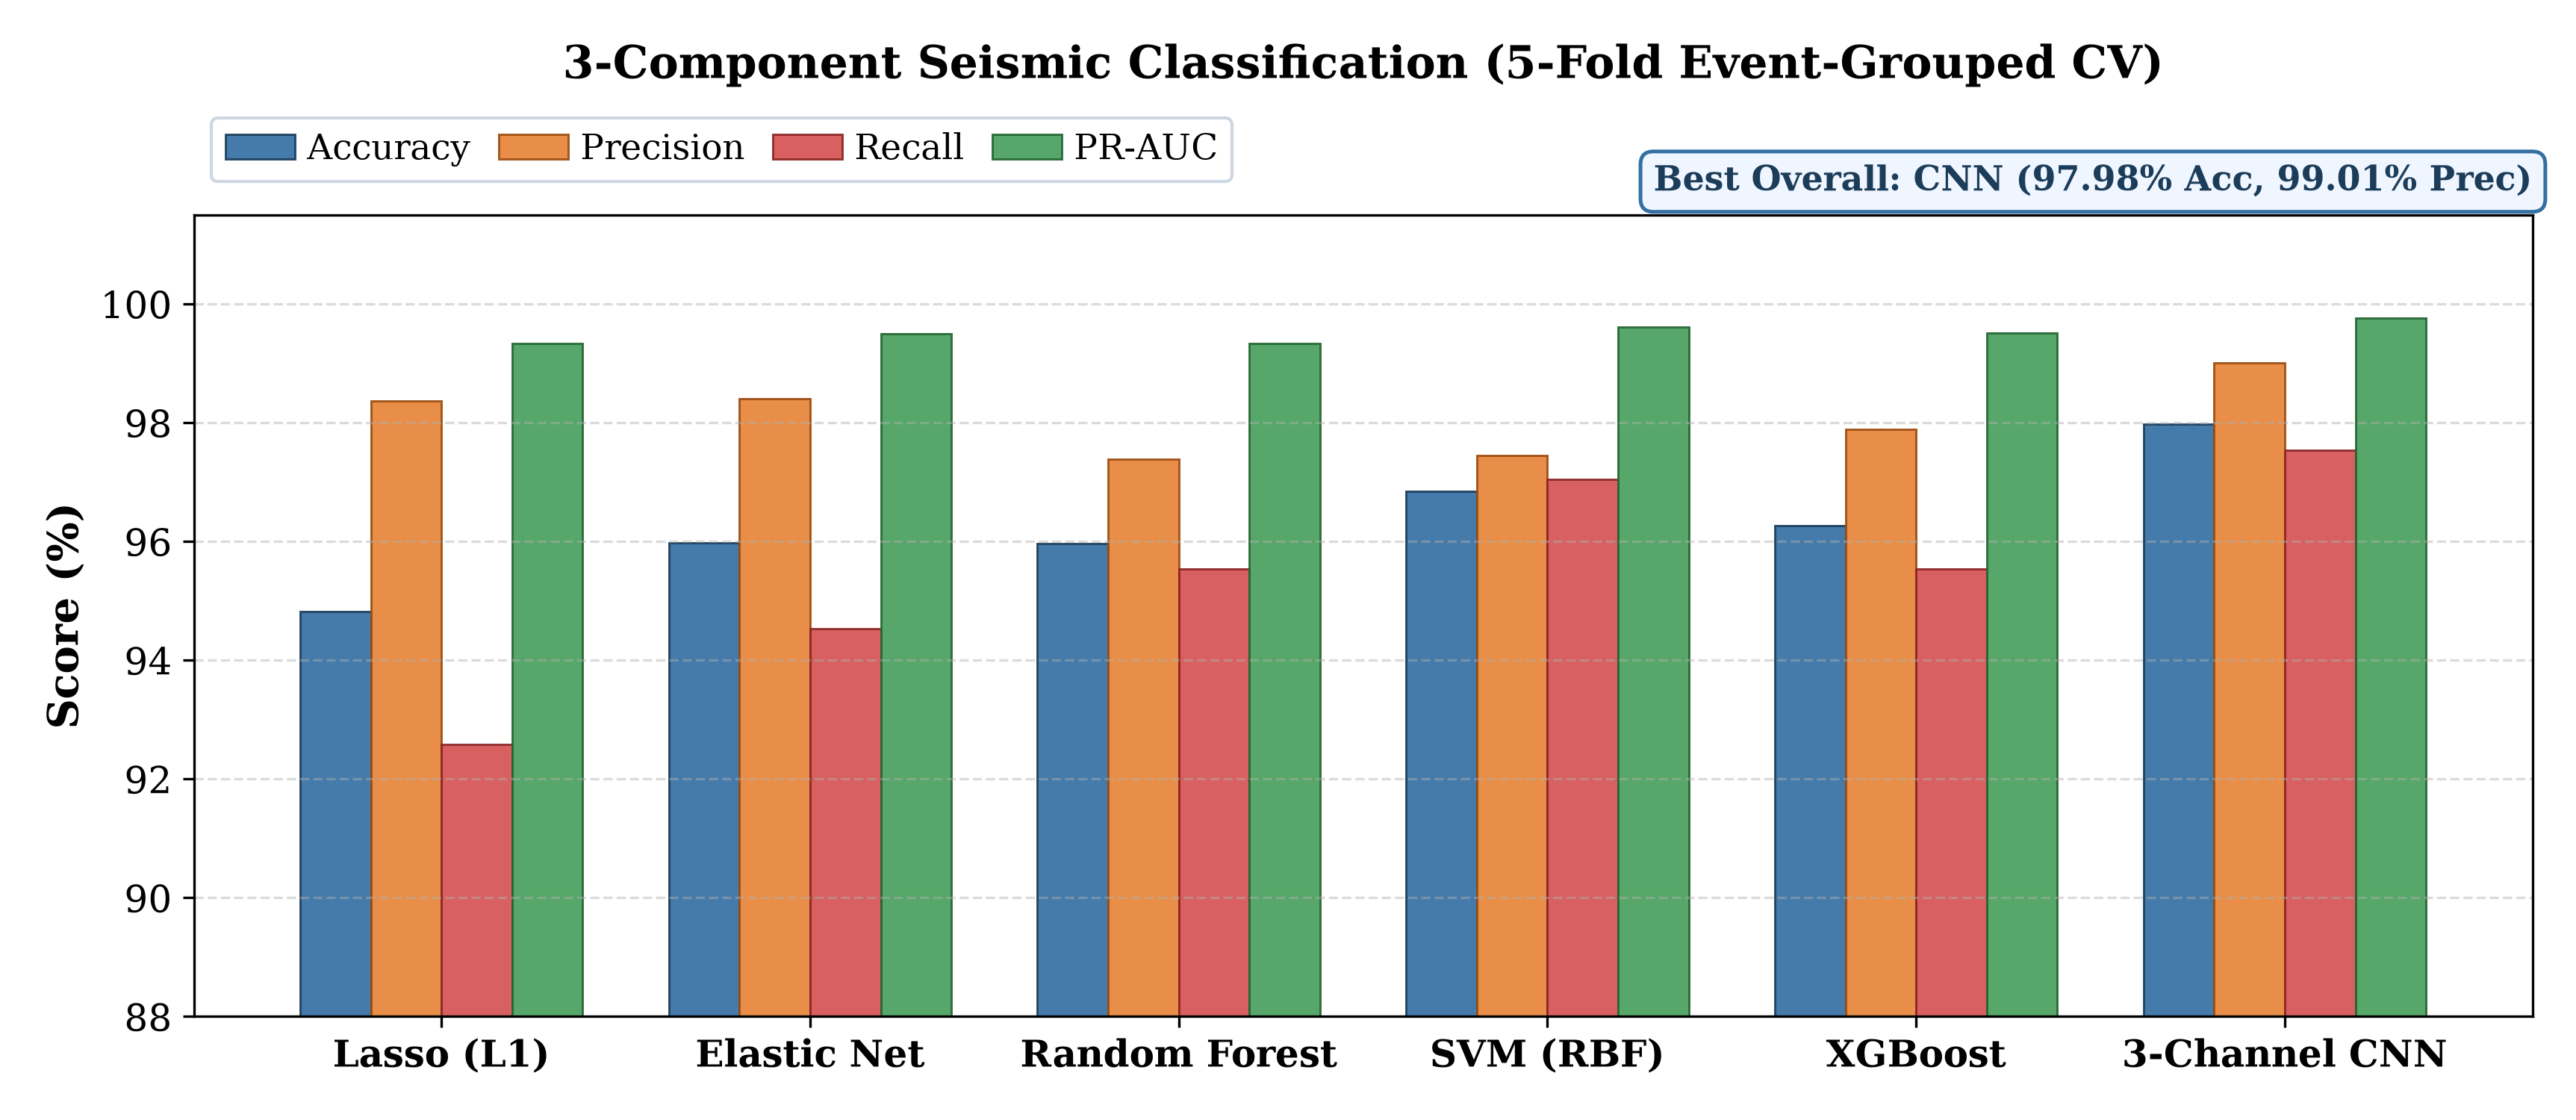
\includegraphics[width=\textwidth, height=5.35cm, keepaspectratio]{model_benchmark_bars.png}\\[0.15em]
  \small \color{navy}\textbf{Key Finding:} \textit{All 6 models achieve $>94\%$ accuracy; the 3-Channel 2D CNN leads across all evaluation metrics (97.98\% Acc, 99.01\% Prec, 99.76\% PR-AUC).}
\end{frame}

% ==============================================================================
% SLIDE 14: FEATURE IMPORTANCE (Plot & Concise Notes)
% ==============================================================================
\begin{frame}{Feature Importance: What Drives Model Decisions?}
  \vspace*{0.05cm}
  \begin{columns}[c,onlytextwidth]
    \begin{column}{0.53\textwidth}
      \centering
      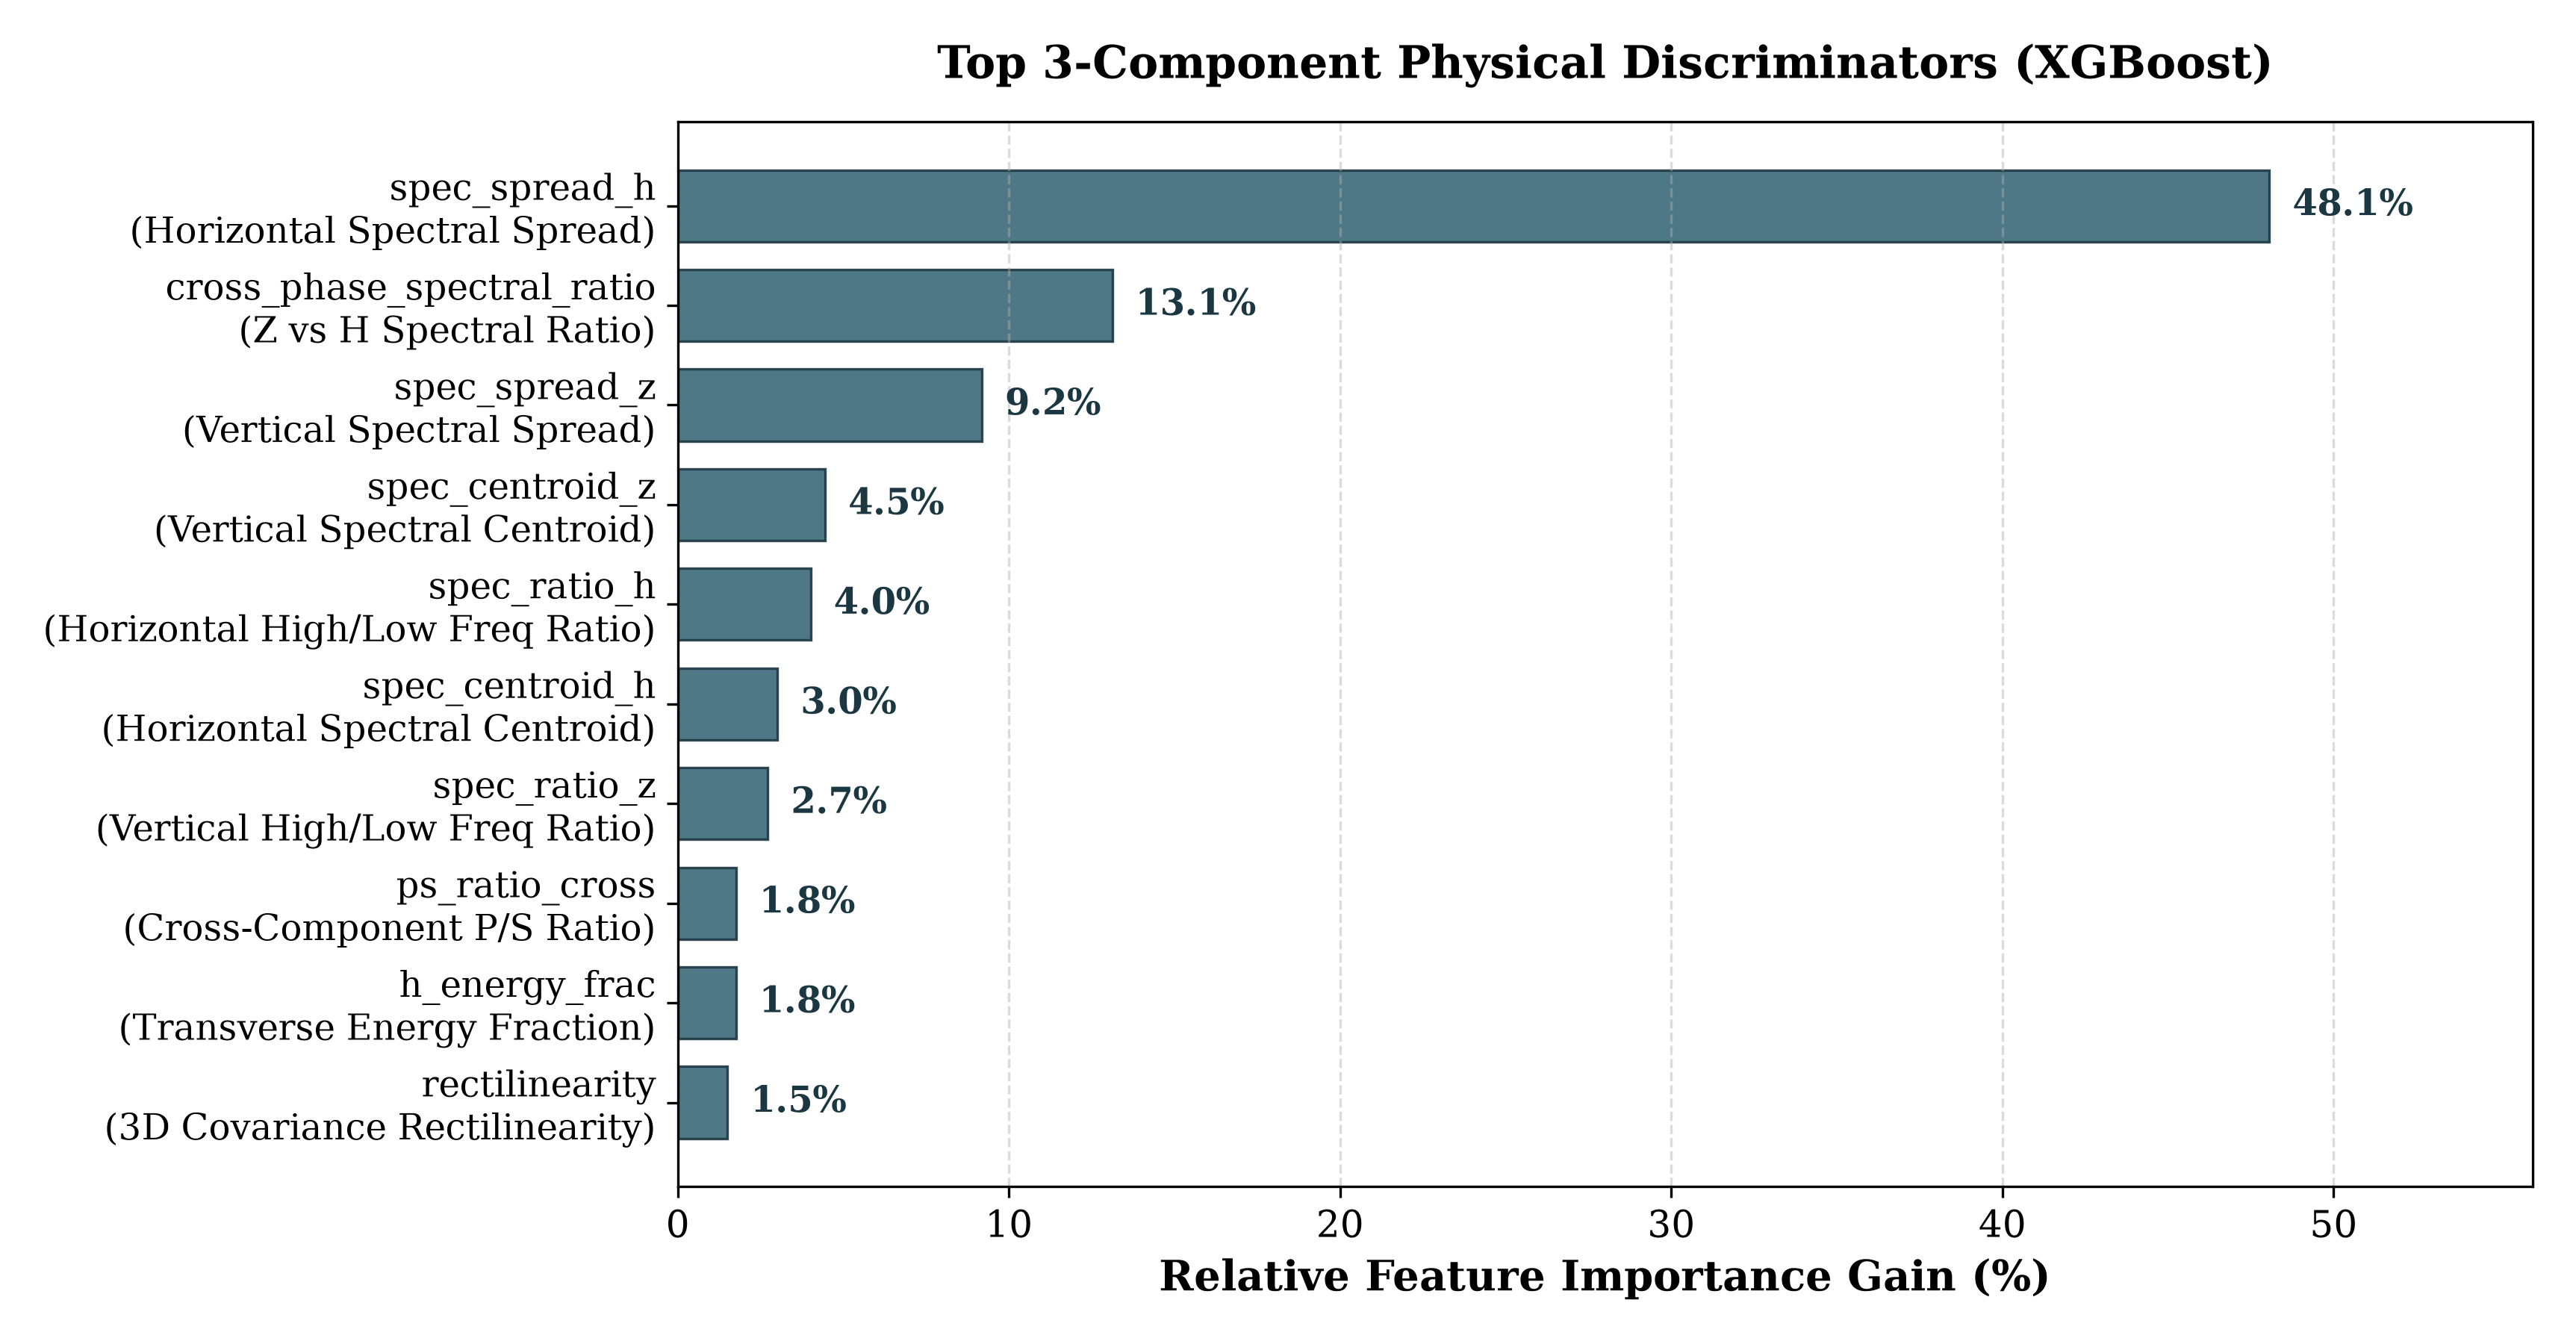
\includegraphics[width=\textwidth, keepaspectratio]{feature_importance.png}
    \end{column}
    \hfill
    \begin{column}{0.44\textwidth}
      \textbf{\color{blastred}\large 48.1\%} \textbf{\color{navy}\small Horizontal Spread}\\[0.15em]
      \footnotesize Earthquakes produce broad horizontal shear motion; explosions show narrow, concentrated horizontal signals.\\[0.8em]

      \textbf{\color{navy}\large 13.1\%} \textbf{\color{navy}\small Vertical-to-Horizontal Ratio}\\[0.15em]
      \footnotesize Explosions are dominated by initial vertical compressional motion; earthquakes produce substantial horizontal energy.\\[0.8em]

      \textbf{\color{tealaccent}\large 9.2\%} \textbf{\color{navy}\small Vertical High Frequencies}\\[0.15em]
      \footnotesize Compact blast sources concentrate energy at higher frequencies than large fault ruptures.
    \end{column}
  \end{columns}
\end{frame}

% ==============================================================================
% SLIDE 15: SECTION 4 DIVIDER
% ==============================================================================
{
\setbeamercolor{background canvas}{bg=navy}
\begin{frame}[plain]
  \vspace*{1.15cm}
  {\fontsize{13}{16}\selectfont \color{tealaccent} SECTION 04}\\[0.4em]
  {\fontsize{24}{28}\selectfont \textbf{\color{white} External Generalization: North Korea (2006--2017)}}\\[0.8em]
  {\fontsize{12}{15}\selectfont \color{slate} Testing model generalization against six declared DPRK underground nuclear tests}\\[1.0em]
  {\fontsize{10}{13}\selectfont \color{slate} Note: DPRK stands for the Democratic People's Republic of Korea (North Korea).}
\end{frame}
}

% ==============================================================================
% SLIDE 16: NORTH KOREA VISUAL CLIMAX
% ==============================================================================
\begin{frame}{External Validation: 100\% Detection Across All 6 DPRK Tests}
  \vspace*{0.05cm}
  \centering
  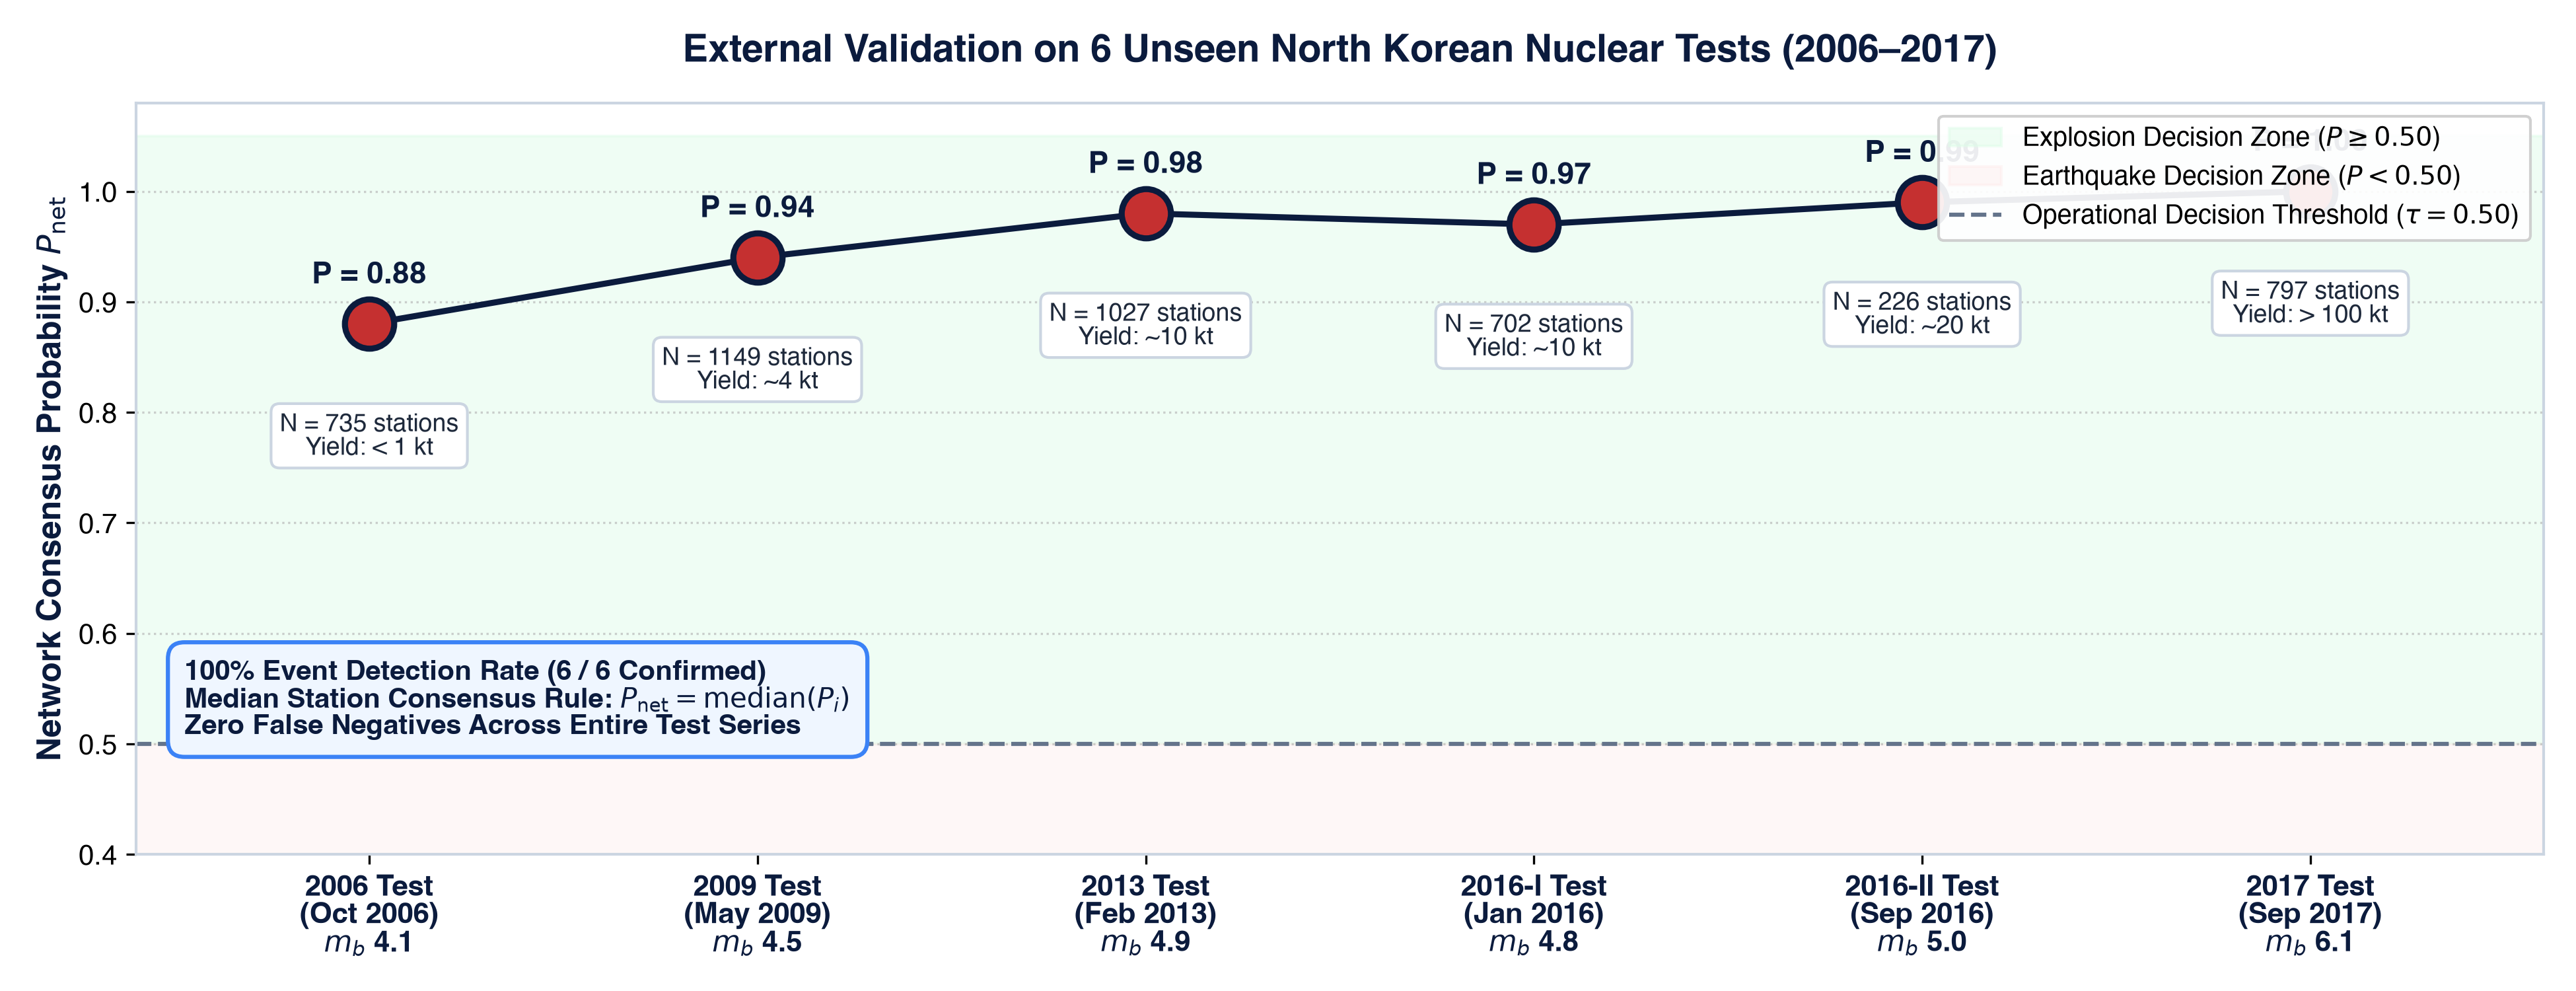
\includegraphics[width=0.96\textwidth, height=4.95cm, keepaspectratio]{dprk_timeline.png}\\[0.2em]
  \small \color{navy}\textbf{Zero False Negatives:} \textit{All 6 unseen nuclear tests classified with high confidence ($P_{\mathrm{net}} \ge 0.88$). These events were completely withheld from model training and hyperparameter tuning.}
\end{frame}

% ==============================================================================
% SLIDE 17: OPERATIONAL REALITY & MULTI-STATION CONSENSUS
% ==============================================================================
\begin{frame}{Operational Reality: Multi-Station Consensus \& Class Imbalance}
  \centering{\normalsize \color{slate} Transitioning from single-sensor models to operational network monitoring.}\par
  \vspace*{0.4cm}

  \begin{columns}[T,onlytextwidth]
    \begin{column}{0.485\textwidth}
      \textbf{\color{navy} Multi-Station Median Consensus}
      \vspace*{0.3em}
      \begin{itemize}\small
        \item Single sensor traces suffer from local noise and signal attenuation.
        \item Global monitoring networks record each event across hundreds of stations ($N = 226$ to $1,149$).
        \item \textbf{Network Decision:} $P_{\mathrm{net}} = \mathrm{median}_{i}(P_i)$.
        \item Aggregation cancels uncorrelated local noise, driving robust $\mathbf{100\%}$ event detection across all tests.
      \end{itemize}
    \end{column}
    \hfill
    \begin{column}{0.485\textwidth}
      \textbf{\color{blastred} The Class Imbalance Challenge}
      \vspace*{0.3em}
      \begin{itemize}\small
        \item Natural earthquakes outnumber nuclear tests by $> 100,000 : 1$.
        \item In extreme imbalance, a $1\%$ single-station false-positive rate yields frequent false alarms:
          \\[0.4em]
          \scriptsize
          $P(\text{Blast} \mid +) = \frac{\text{TPR} \cdot \pi}{\text{TPR} \cdot \pi + \text{FPR} \cdot (1 - \pi)}$
          \\[0.4em]\small
        \item Requiring multi-station network consensus pushes false alarms toward zero, enabling reliable monitoring.
      \end{itemize}
    \end{column}
  \end{columns}
\end{frame}

% ==============================================================================
% SLIDE 18: TAKEAWAYS & CONCLUSIONS
% ==============================================================================
{
\setbeamercolor{background canvas}{bg=navy}
\begin{frame}[plain]
  \vspace*{0.6cm}
  {\fontsize{13}{16}\selectfont \color{tealaccent} SUMMARY \& CONCLUSIONS}\\[0.35em]
  {\fontsize{22}{26}\selectfont \textbf{\color{white} Key Takeaways for Statistical Monitoring}}\\[0.8em]

  \begin{columns}[T,onlytextwidth]
    \begin{column}{0.315\textwidth}
      {\normalsize \textbf{\color{tealaccent} 1. Feature Engineering}}\\[0.3em]
      {\color{white}\small Combining 18 energy ratios and spectral decay metrics yields $>96\%$ accuracy with classical classifiers while strictly preventing geographic data leakage.}
    \end{column}
    \hfill
    \begin{column}{0.315\textwidth}
      {\normalsize \textbf{\color{tealaccent} 2. Representation Learning}}\\[0.3em]
      {\color{white}\small 2D STFT spectrograms allow CNNs to learn directly from time-frequency images without manual thresholds, leading the benchmark ($97.98\%$ Acc, $0.9976$ PR-AUC).}
    \end{column}
    \hfill
    \begin{column}{0.315\textwidth}
      {\normalsize \textbf{\color{tealaccent} 3. Operational Consensus}}\\[0.3em]
      {\color{white}\small Multi-station median voting overcomes extreme natural class imbalance, successfully identifying all 6 North Korean nuclear tests with zero false negatives.}
    \end{column}
  \end{columns}

  \vspace*{1.0cm}
  \centering
  {\fontsize{14}{18}\selectfont \color{white} \textbf{Thank You}}
\end{frame}
}

\end{document}
